\documentclass[rep.tex]{subfiles}
\begin{document}

\chapter{Zadanie 17}
\label{zad17}
\section{Treść}
Zaprojektować czebyszewowski filtr pasmowo przepustowy (FPP, rys.~\ref{fig:zad17:cheb}) o strukturze
paskowej jak na rys.~\ref{fig:zad17:strip} dla następujących danych: $Z_0 = 50~\Omega$, $f_0 = 2.8 \times 10^9~Hz$, $w = 0.1$,
$L_r = 0.2~dB$, $f_a = 3.2 \times 10^9~Hz$ i $L_a = 30~dB$.
Filtr zrealizować z odcinków symetrycznej linii paskowej opisanej w zadaniu~\ref{zad4}.

\begin{figure}[!htbp]
  \centering
  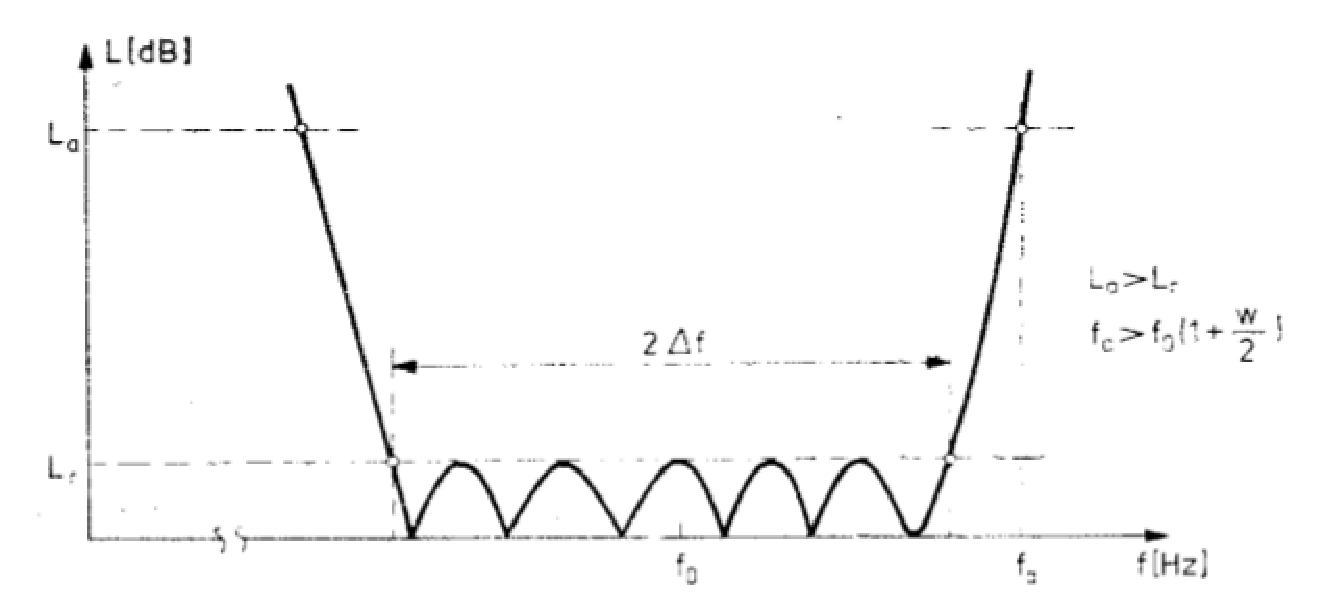
\includegraphics[scale=0.5]{fig/zad17/cheb}
  \caption{Charakterystyka projektowanego filtru}
  \label{fig:zad17:cheb}
\end{figure}

\begin{figure}[!htbp]
  \centering
  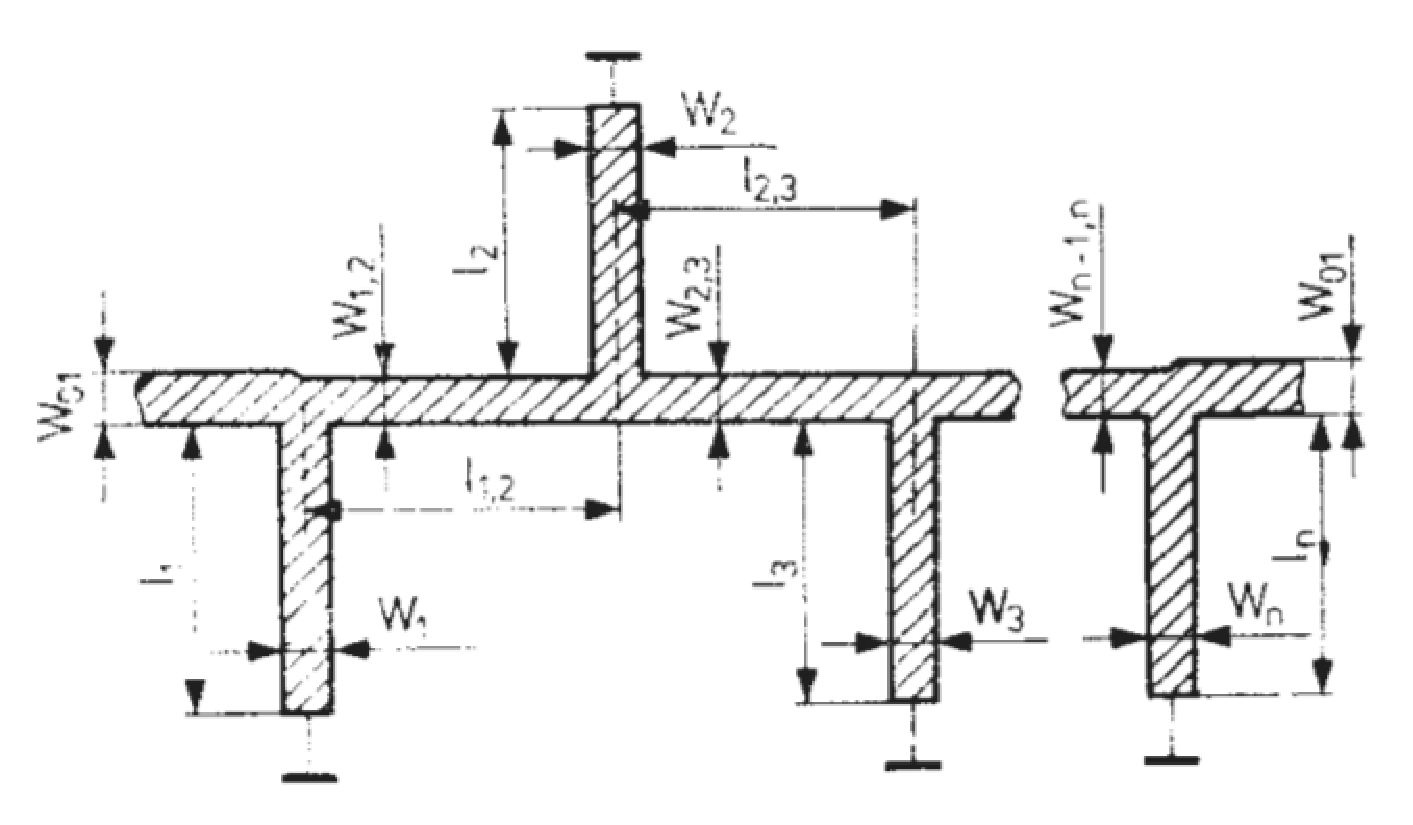
\includegraphics[scale=0.5]{fig/zad17/strip}
  \caption{Realizacja filtru przy użyciu symetrycznej linii paskowej}
  \label{fig:zad17:strip}
\end{figure}

\section{Rozwiązanie}
W pierwszym kroku należy obliczyć minimalną ilość sekcji filtru:
\begin{align}
  n &\geq \frac{arch \sqrt{\frac{L_a' - 1}{L_r' - 1}}}{arch \Bigg(\frac{\sin\frac{\pi w_a}{4}}{\sin\frac{\pi w}{4}}\Bigg)} \\
  &= 4 \nonumber
\end{align}

Następnie należy obliczyć parametry filtru dolnoprzepustowego a na ich podstawie wartości elementów filtru o parametrach skupionych.
Wyniki tych obliczeń przedstawia tabela~\ref{tab:zad17:params}.

\begin{table}
  \centering
  \caption{Parametry zaprojektowanego filtru}
  \label{tab:zad17:params}
  \begin{tabular}{l l l l l l l}
    \hline\hline
    i & g & $Z_0$ [$\Omega$] & $w$ [mm] & $l$ [mm]\\
    \hline
    0 & 1.0           &               &               &               \\
    1 & 1.30287657175 & 3.20338115776 & 47.5830406797 & 16.7294898437 \\
    2 & 1.28442456136 & 3.46442342228 & 43.8597176927 & 16.7294898437 \\
    3 & 1.97619882964 & 3.39627708893 & 44.7764554109 & 16.7294898437 \\
    4 & 0.84680075915 & 4.9956490685  & 29.8615873107 & 16.7294898437 \\
    5 & 1.0           &               &               &               \\
    \hline\hline
  \end{tabular}
\end{table}
\end{document}
